% Drawing 43/04-11 -- folder 43, batch 04, archive page 65 (PDF page 66).
% Transcription: à gauche, un croquis : un parallélogramme étroit, ses deux longs côtés repassés en gras, le sommet du haut marqué $\mathfrak{m}$ et celui du bas $\mathfrak{p}$.
% Kind: narrow parallelogram with vertices m and p. Method 2 (schematic redraw from the facsimile). Status: ok.
% Notes: Ink. A narrow parallelogram standing on its point: the two long sides heavy, the two short sides thin and not quite closed on the page (drawn closed), a dot and the gothic m at the top, a dot and the gothic p at the bottom. The word « Hom » under it is text. Redrawn 2026-11-12 (issue 128): to check again.
% Coordinates: 1 unit = 1 mm = 1/100 of the crop width, y downwards as on the crop (bbox in page fractions: [0.12, 0.42, 0.32, 0.57]).
% Redrawn by Claude (claude-fable-5-2), issue #128, 2026-11-12; not checked by a human; not compiled (no TeX in the session).
% Rights: reproduces part of the work -- behind RENDER_TRANSCRIPTS, never published by itself.
\documentclass[tikz,border=3pt]{standalone}
\usepackage{amsmath,amssymb}
\usetikzlibrary{patterns,arrows.meta}
\tikzset{pencil/.style={black!45}, struck/.style={black!35}, mpt/.style={circle,draw,inner sep=1.3pt}, pt/.style={circle,fill,inner sep=0.9pt}, opt/.style={circle,draw,fill=white,inner sep=1.1pt}, Rd/.style={red!75!black}, Gn/.style={green!45!black}, Br/.style={brown!70!black}}
\begin{document}
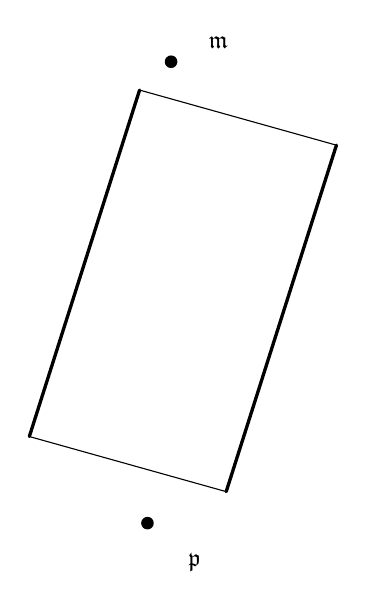
\begin{tikzpicture}[x=1mm,y=-1mm,line cap=round,line join=round,font=\small]
\coordinate (a) at (51,25);
\coordinate (b) at (76,32);
\coordinate (c) at (62,76);
\coordinate (d) at (37,69);
\draw[very thick] (a) -- (d);
\draw[very thick] (b) -- (c);
\draw (a) -- (b);
\draw (d) -- (c);
\fill (55,21.4) circle [radius=0.8];
\fill (52,80) circle [radius=0.8];
\node at (61,19) {$\mathfrak{m}$};
\node at (58,85) {$\mathfrak{p}$};
\end{tikzpicture}
\end{document}
